\subsection{Shared-Reference Replay}\label{app:shared_replay}

The earlier one-encoder controls either restrict a common feature interface
or learn a replacement readout. Shared-reference replay retains a different
object: the healthy input-to-output function on a separate output path. Its
current features need not support the old weights. The reference parameters
remain available, but their dense computation is shared with the current
model. This access condition differs from repairing terminal features alone.
No old-label or distillation loss is added to continuation.

For a width-$m$ two-nonlinearity trunk, first-map changes have row support
$S$, $|S|=k$, and the second-map change is $UV$ of rank at most $r$.
Proposition~\ref{prop:shared_replay} evaluates both nonlinearities without
linearizing the update. The final affine encoder map and current task head
remain trainable; their product is folded for native serving. The healthy
final affine map can similarly be folded into the old head. One healthy
dense first and second map is stored, along with sparse/low-rank updates
and both heads. The serving package omits a second full encoder.
Extra multiply--accumulates (MACs), excluding biases and elementwise work,
are $kd+km+2rm+Cm$ for input dimension $d$ and $C$ old outputs.
For the selected HAR and SNR configurations these are $3{,}396$ and
$6{,}848$, respectively: $8.4\%$ and $32.3\%$ above the merged current
network. Measured latency differs substantially from these arithmetic ratios.

Low-rank parameters alone do not give a low-rank activation difference.
For $n$ scalar inputs $x_i=i$, take $W_1^0=0$, biases
$b_j=-(j-\tfrac12)$, and the rank-one update $\Delta W_1=\mathbf1$.
The healthy ReLU activations vanish, whereas the change matrix has entries
$\max\{i-j+\tfrac12,0\}$. It is lower triangular with diagonal $1/2$
and hence has rank $n$. Row support supplies the invariant used in our
construction: after any coordinatewise nonlinearity, $\delta a_1$ is still
supported on $S$. This explains the hybrid restriction; it is not a lower
bound against every possible implementation of dense low-rank updates.

The same identity applies to an identity residual block with fixed
normalization. Updating $k$ output channels of its first convolution confines
the activation difference to those channels. A $3\times3$ rank-reducing
convolution followed by a $1\times1$ expansion represents the second update.
Adding the unchanged shortcut and applying ReLU gives the merged current
block in real arithmetic. Before the visual study, fixed BN is folded into
the healthy convolutions; this defines the numerical reference from the start.

\subsection{Dense Replay, Support and Update Rank}\label{app:shared_replay_rank}

Row support is one admissible structure, not the only one. Replace the first map
by $W_1^0+PQ$ with $P\in\mathbb R^{m\times s}$, $Q\in\mathbb R^{s\times d}$, the
second by $W_2^0+UV$ of rank $r$, and add biases $\delta b_1,\delta b_2$. With
$a_1=\sigma(W_1^0x+b_1^0+PQx+\delta b_1)$ and $a_1^0=\sigma(W_1^0x+b_1^0)$,
substitution into $(W_2^0+UV)a_1+b_2^0+\delta b_2$ gives
\begin{equation}
 t_2=t_2^0+W_2^0(a_1-a_1^0)+UVa_1+\delta b_2
 \label{eq:dense_replay}
\end{equation}
exactly, for any coordinatewise $\sigma$. The correction is dense, so the extra
MACs above the folded current-only graph are $sd+ms+m^2+2rm+n_cm$:
the saving comes from reusing the healthy dense
products, not from sparsity.

For each
saved full-joint endpoint we truncate the first- and second-map deltas by SVD,
keep everything else fixed, and score the official test split
(Table~\ref{tab:rank}). A truncated update is a member of the dense low-rank
family, so a nonnegative gap proves that this structure can reproduce joint
accuracy. A negative gap does not prove that no trained member can: the trained
rank-$16/12$ SNR arm below reaches parity although rank $32$ is needed to
reach the same accuracy tolerance when truncating this particular first-map
update. This retrospective projection does not identify a necessary rank
for a trained family or explain the sparse-to-dense gain by rank alone.

\begin{table}[h]
\centering
\small
\caption{Mean accuracy difference, in points, to the saved full-joint endpoint
after truncating its first-map ($s$) or second-map ($r$) update and scoring the
official test split. Ten endpoints per task. A truncated update is a member of
the dense low-rank family, so a nonnegative gap is achievable accuracy, not a
lower bound on the family.}
\label{tab:rank}
\begin{tabular}{lcc}
\toprule
Update kept & HAR & SNR\\
\midrule
first map, $s=16$ & $-0.13$ & $-0.56$\\
first map, $s=32$ & $-0.07$ & $-0.01$\\
second map, $r=16$ & $-0.18$ & $-0.16$\\
second map, $r=24$ & -- & $+0.01$\\
$(s,r)=(16,16)$ & $-0.28$ & --\\
$(s,r)=(32,24)$ & -- & $-0.02$\\
\bottomrule
\end{tabular}
\end{table}

Development selected $(16,12)$ for SNR, the smallest grid configuration clearing
the predeclared gate on seeds $800$--$802$. Ten fresh seeds then give a primary
gain of $\DenseSnrGain$ points $[\DenseSnrGainLow,\DenseSnrGainHigh]$ over
detachment, a difference of $\DenseSnrFull$ points
$[\DenseSnrFullLow,\DenseSnrFullHigh]$ to ordinary joint training, and an
auxiliary MSE ratio of $\DenseSnrMse$
$[\DenseSnrMseLow,\DenseSnrMseHigh]$. Accuracies are $\DenseSnrDetAcc\%$,
$\DenseSnrJointAcc\%$ and $\DenseSnrFullAcc\%$. Every observed consumer
disagreement is zero, every certificate meets the five-point budget with maximum
upper bound $0.0092$, the exact reference error is $0$, and packed serving
differs by at most $\DenseMaxPackedError$ logits without changing a merged
prediction.

The HAR gate rejects the same family: primary differences are $\DenseHarDevLow$
to $\DenseHarDevHigh$ points on development while reconstruction improves, so no
HAR configuration was confirmed. Extra capacity is not a free improvement; it
improves this SNR endpoint but reduces HAR accuracy under the specified
recipe. The sparse HAR arm and its confirmed
reconstruction result are unchanged.

The matched SNR current-only graph costs $21{,}184$ MACs after folding its
final affine map into the primary head. Dense replay adds $11{,}456$ MACs
($54.1\%$), versus $6{,}848$ ($32.3\%$) for sparse replay. The earlier
$12{,}288$ count mixed an extra head already present in the current baseline
with $128$ bias additions and divided by the unfused $24{,}576$-MAC encoder;
we retain that historical record and use the matched graph here. Neither
an SVD projection nor this chosen program supplies a lower bound on all
compatible implementations. Measured latency is reported separately in
Appendix~\ref{app:shared_replay_cost}.

Layerwise update rank also depends on the parameterization. The standard
positive-rescaling symmetry of ReLU networks~\citep{dinh2017sharp} gives a
simple check: $(W_1,b_1,W_2,b_2)\mapsto(2W_1,2b_1,W_2/2,b_2)$ preserves
the function, while both matrix differences can have full row rank.
Our SVD results therefore concern saved updates in fixed coordinates,
rather than an intrinsic rank of the learned function. The support/rank
factorial in Appendix~\ref{app:frontier_factorial} measures the distinction
directly under matched future training orders.

\subsection{Development, Selection and Fresh Confirmation}\label{app:shared_replay_protocol}

The fixed plan precedes development and is included with its source hashes.
Development uses saved healthy checkpoints, optimizer states and fitting/
validation splits for seeds $800$--$802$ on both tasks. The four configurations
are $(k,r)\in\{(0,4),(4,4),(8,8),(16,8)\}$. On $1{,}024$ fitting inputs,
the original joint-loss gradient ranks first-map rows and initializes the
right second-map factors from its singular vectors. Update amplitudes start
at zero. This training-only initialization rule is fixed before outcomes.
The paired detached and joint arms share support, factors, inherited moments,
and future minibatches. New update parameters start with zero Adam moments.
We retain the original unclipped Adam, learning rate $10^{-3}$, batch $256$,
$30/25$ HAR/SNR epochs, doses $100/1$, and $10\%/20\%$ primary labels.

Development requires every old-contract disagreement to be at most $1\%$.
HAR additionally requires mean reconstruction ratio at most $0.95$ and mean
primary difference at least $-0.5$ points; SNR requires a positive paired
primary-gain interval and mean accuracy within $0.5$ points of unrestricted
joint training. Eligible configurations are ranked by extra MACs. This
selects HAR $(4,4)$ and SNR $(16,8)$. No test score enters selection.

The native development cost screen fails the registered batch-$1/1024$
limits of $1.20/1.10$. This failure is recorded before confirmation; the
fixed plan permits a partial utility/compatibility frontier. Twenty new warm
checkpoints, seeds $2500$--$2509$ on each task, then train the frozen
structured pair and ordinary full-update detached/joint controls. These are
new training seeds on the existing data splits, not new populations.
Fresh $1{,}024$-input monitors use RNG $10700001+\text{seed}$, plus $100000$
for HAR, and tail probability $0.05/600$. Each evaluates classification and
two fixed confidence thresholds calibrated on healthy fitting features.
Certificates concern the finite test-corpus remainder with a five-point
budget. Utility intervals are paired, two-sided $95\%$ $t$ intervals over
all ten seeds; the criteria and cost limits are unchanged.

\begin{table}[t]
\centering
\caption{Fresh shared-replay confirmation, ten seeds per task. J--D compares
the matched structured arms. Intervals are paired $95\%$ $t$ intervals;
accuracy differences use percentage points. Every old class/selective
consumer certifies, but SNR misses noninferiority to full joint training.}
\label{tab:shared_replay}
\small
\begin{tabular}{lcc}
\toprule
Outcome & HAR $(k,r)=(4,4)$ & SNR $(16,8)$ \\
\midrule
Primary J--D & $\ReplayHarGain$ & $+\ReplaySnrGain$ \\
$95\%$ interval & $[\ReplayHarGainLow,\ReplayHarGainHigh]$ & $[\ReplaySnrGainLow,\ReplaySnrGainHigh]$ \\
Reconstruction/regression MSE J/D & $\ReplayHarMse$ & $0.817$ \\
$95\%$ interval & $[\ReplayHarMseLow,\ReplayHarMseHigh]$ & $[0.782,0.853]$ \\
Primary J--full J & $-0.024$ & $\ReplaySnrFull$ \\
$95\%$ interval & $[-0.689,0.641]$ & $[\ReplaySnrFullLow,\ReplaySnrFullHigh]$ \\
Class / selective certificates & $20/20$ each & $20/20$ each \\
Maximum old decision disagreement & $0$ & $0$ \\
\bottomrule
\end{tabular}
\end{table}


HAR confirms reconstruction progress and primary noninferiority relative
to its structured detached arm. SNR confirms positive auxiliary transfer,
but misses the half-point noninferiority criterion against full joint
training. The unrestricted SNR pair gains $1.073$ points; the structured
pair gains $\ReplaySnrGain$. Both nonlinear layers change their parameters
and observed ReLU gates. All $120$ old-contract bounds pass, with no
observed decision changes. The largest remaining-disagreement bound is
$1.092\%$ on HAR and $0.917\%$ on SNR. These findings establish useful
learning with class and selective compatibility, while leaving a cost
failure and an SNR capacity cost.

The dense companion study was registered separately before its outcomes. Its
grid is $(s,r)\in\{(16,12),(24,16),(32,24)\}$; the same development seeds,
warm checkpoints, orders, initialization rule and gate decide selection, and
seeds $2520$--$2529$ confirm the chosen pair. HAR fails the primary gate at all
three configurations, so only SNR is confirmed, at $(16,12)$. No criterion was
changed after any outcome.

The full reference path reproduces stored healthy logits exactly under
the declared evaluation arithmetic. The compressed native-float32 old
heads have maximum errors $1.27\times10^{-5}$ on HAR and
$8.84\times10^{-6}$ on SNR; their actual decisions are the ones monitored.
An independent raw-state replay verifies all $40$ structured endpoints and
$120$ contracts. Packed and independently merged current serving differ by
at most $1.53\times10^{-5}$, with two near-tied current classifications
changing across all replayed endpoints. Thus the algebraic identity is not
a claim of bitwise equality after floating-point reassociation. Reported
utility uses the actual packed two-output implementation.

\subsection{Native Serving and Strong Reuse Controls}\label{app:shared_replay_cost}

An isolated four-thread CPU process measures both arms of all six selected
development endpoints. Both outputs use float32; the merged current-only
baseline folds the same final affine maps and emits the same current
function in real arithmetic. We compare eager and TorchScript serving,
two independently evaluated functions, and a stronger control sharing the
healthy first map but recomputing both dense second maps. Packed replay
combines small products before serving. Each measurement warms all paths,
alternates operation order, and retains $71$ repetitions. Table~\ref{tab:replay_cost}
reports medians across the six paired endpoint measurements per task.

\begin{table}[h]
\centering
\caption{Isolated float32 TorchScript inference, four CPU threads. Times
are microseconds per batch; Replay/current is the median paired ratio.
Prefix shares the healthy first map and recomputes both second maps.
The registered limits are $1.20\times$ at batch $1$ and $1.10\times$ at $1024$.}
\label{tab:replay_cost}
\small
\begin{tabular}{lrrrrrr}
\toprule
Task & Batch & Current & Replay & Prefix & Independent & Replay/current \\
\midrule
HAR & 1 & 20.6 & 45.3 & 43.4 & 40.1 & $2.20\times$ \\
HAR & 1024 & 276.1 & 508.3 & 508.9 & 543.9 & $1.81\times$ \\
SNR & 1 & 16.8 & 42.7 & 39.5 & 32.4 & $2.54\times$ \\
SNR & 1024 & 157.2 & 324.7 & 352.7 & 312.4 & $2.07\times$ \\
\bottomrule
\end{tabular}
\end{table}


Kernel launches, strided intermediates and small products dominate these
small networks. At batch $1$, sharing fewer arithmetic operations is slower
than evaluating two independently folded functions. At batch $1024$, HAR
replay is modestly faster than that control; SNR replay is slower. A separate
fixed-shape Inductor experiment on the joint seed-$800$ states yields
matched packed/current ratios $1.44/1.46$ for HAR and $1.50/1.73$ for SNR
at batch $1/1024$, still above budget. Its current-only batch-$1$ latencies
are $41.8/38.9\,\mu$s, slower than TorchScript's $20.6/16.8\,\mu$s.
Initial setup ranges from $0.10$ to $13.88$ seconds across compiled paths.
Both absolute times and ratios are retained; the smaller compiled ratio
does not establish a faster deployment. No universal latency claim follows
from the exact identity or MAC count.

The same protocol on the ten dense SNR endpoints gives median packed/current
ratios of $3.02$ at batch $1$ and $2.57$ at batch $1024$ under TorchScript
($3.22/2.63$ eager), against $2.54/2.07$ for the sparse arm. Denser corrections
raise both the analytic MAC count and the measured cost, so the dense arm is
reported as the utility endpoint of the frontier, not as a deployment proposal.
For a fixed input dimension of $561$, the same sparse implementation improves
from $1.53\times$ at width $64$ to $1.12\times$ at width $1024$ for batch $1024$,
and remains between $1.56\times$ and $4.70\times$ at batch $1$; the batch-$1$
target is not met by any measured two-output path at these widths.

\subsection{ResNet-18 Capacity Boundary}\label{app:shared_replay_vision}

The prospective ImageNet-V1 ResNet-18/CIFAR-100 screen uses $64\times64$
images, $42{,}952$ fitting, $5{,}000$ validation and $2{,}048$ isolated
anchor images, and a fixed $20\%$ fine-labeled fitting mask. Healthy fine-100
and coarse-20 heads use the same labeled subset. Coarse labels are not used
in continuation; their derivability from fine labels is explicit. Earlier
blocks and normalization are fixed; only the last identity-residual block
can change. Current-head normalization remains fixed to healthy labeled
features. Three AdamW epochs use identical original fitting-index orders,
batch $128$, head learning rate $10^{-3}$ and weight decay $10^{-4}$.
The ordinary dense-block control uses learning rate $10^{-4}$.

The initial $(k,r)=(0,8),(8,8),(16,16)$ screen at update rate $10^{-3}$
does not pass the prescribed two-point gain over both healthy and head-only
accuracy, with a half-point tolerance against the dense control. A second
fixed capacity screen, declared before execution, tests $(64,32),(128,64),
(256,128)$ at the dense block's update rate $10^{-4}$. Figure~\ref{fig:replay_vision}
retains all six outcomes. The largest configuration reaches $45.30\%$,
against $43.74\%$ healthy, $43.48\%$ head-only and $45.74\%$ dense.
Its $1.56$-point net gain still misses the fixed two-point gate. Every old
decision is unchanged, but neither screen proceeds to more development
seeds or official test scoring. A folded-bias gradient initialization error
before the first continuation is retained as a technical failure, separately
from these completed scientific outcomes.

\begin{figure}[t]
\centering
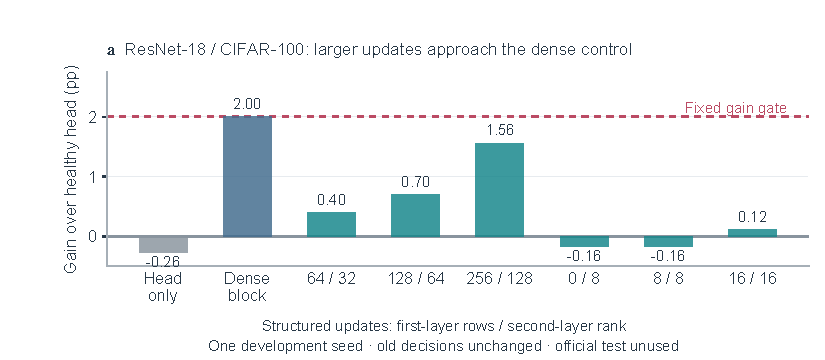
\includegraphics[width=\linewidth]{figures/fig_replay_vision.pdf}
\caption{All six ResNet-18 shared-replay capacity candidates at seed $2600$.
Bars show validation accuracy gain over the healthy fine head. The dense
last-block control reaches the fixed two-point gate; the structured updates
do not. The two grids use their prospectively fixed update rates. Old coarse
class and selective decisions are unchanged. This development screen uses
no official test examples and is not an auxiliary-benefit study.}
\label{fig:replay_vision}
\end{figure}
